\subsection{Aplicação Painel: Desativar/Ativar}
\subsubsection*{Descrição do caso de uso}
Desativar um registo significa que este se vai manter na base de dados, mas não irá constar mais nas UI da aplicação de Fábrica. Para desativar/ativar um registo, o utilizador necessita pressionar o botão desativar/ativar na linha referente ao registo que pretende atualizar. Pelo facto de ser apenas uma procedimento executado em background, não possui nenhuma view.

\subsubsection*{Models compatíveis com o caso de uso}
Este caso de uso é compatível com os models Colaboradores, Pontos de Recolha e Clientes.

\subsubsection*{Fluxo do caso de uso}
O caso de uso inicia-se quando o utilizador pressionar o botão desativar/ativar da linha do registo que pretende desativar/ativar. Após executar a ação é apresentada uma mensagem ao utilizador


\begin{figure}[H] 
	\begin{center}
		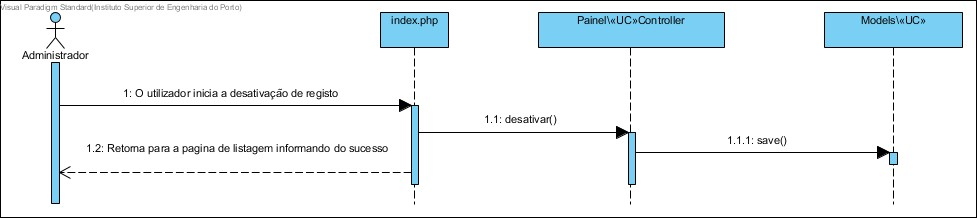
\includegraphics[width=\textwidth,keepaspectratio]{figuras/Diagramas_vp/SD_Painel_5_Desativar.jpg}
		\caption{Diagrama de sequência de desativar/ativar registo}
		\label{fig:sd_desativar} 
	\end{center}
\end{figure}